\documentclass{standalone}
\usepackage{tikz}
\usetikzlibrary{patterns, positioning}


\begin{document}
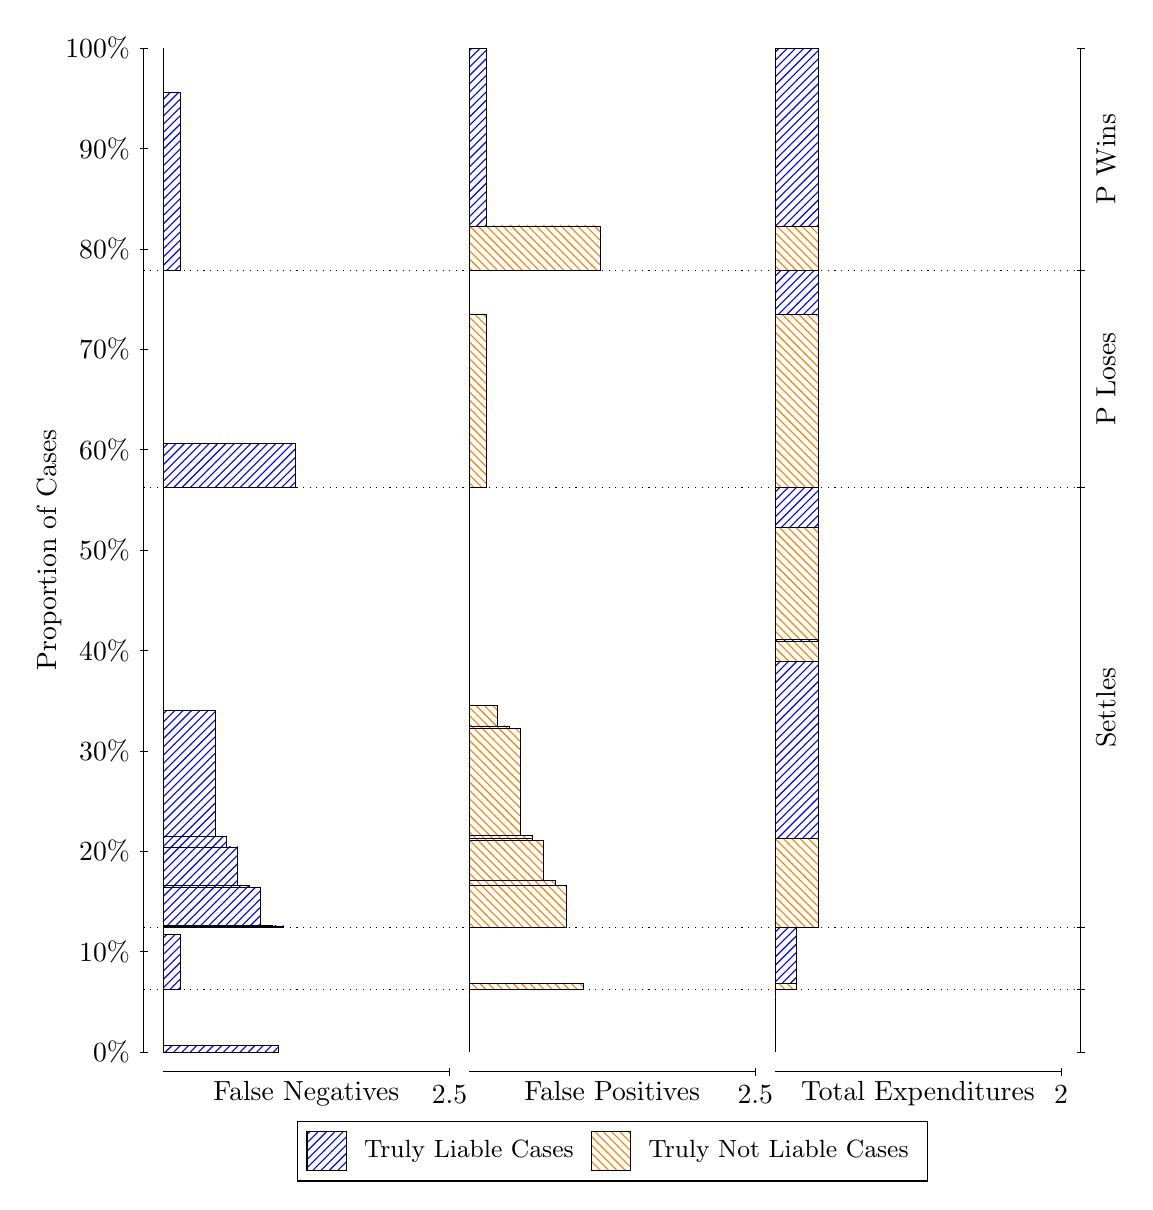
\begin{tikzpicture}
\draw[black, very thin] (1.5,1.75) -- (1.5,14.5);
\node[rotate=90, text=black, anchor=center] at (0.3, 8.125) {Proportion of Cases};
\draw[black, very thin] (1.45,1.75) -- (1.55,1.75);
\node[text=black, anchor=east] at (1.45, 1.75) {0\%};
\draw[black, very thin] (1.45,3.025) -- (1.55,3.025);
\node[text=black, anchor=east] at (1.45, 3.025) {10\%};
\draw[black, very thin] (1.45,4.3) -- (1.55,4.3);
\node[text=black, anchor=east] at (1.45, 4.3) {20\%};
\draw[black, very thin] (1.45,5.575) -- (1.55,5.575);
\node[text=black, anchor=east] at (1.45, 5.575) {30\%};
\draw[black, very thin] (1.45,6.85) -- (1.55,6.85);
\node[text=black, anchor=east] at (1.45, 6.85) {40\%};
\draw[black, very thin] (1.45,8.125) -- (1.55,8.125);
\node[text=black, anchor=east] at (1.45, 8.125) {50\%};
\draw[black, very thin] (1.45,9.4) -- (1.55,9.4);
\node[text=black, anchor=east] at (1.45, 9.4) {60\%};
\draw[black, very thin] (1.45,10.675) -- (1.55,10.675);
\node[text=black, anchor=east] at (1.45, 10.675) {70\%};
\draw[black, very thin] (1.45,11.95) -- (1.55,11.95);
\node[text=black, anchor=east] at (1.45, 11.95) {80\%};
\draw[black, very thin] (1.45,13.225) -- (1.55,13.225);
\node[text=black, anchor=east] at (1.45, 13.225) {90\%};
\draw[black, very thin] (1.45,14.5) -- (1.55,14.5);
\node[text=black, anchor=east] at (1.45, 14.5) {100\%};

\draw[black, very thin] (13.4,1.75) -- (13.4,14.5);
\draw[black, very thin] (13.35,1.75) -- (13.45,1.75);
\node[anchor=west] at (13.35, 1.75) {};
\draw[black, very thin] (13.35,2.5408) -- (13.45,2.5408);
\node[anchor=west] at (13.35, 2.5408) {};
\draw[black, very thin] (13.35,3.3287) -- (13.45,3.3287);
\node[anchor=west] at (13.35, 3.3287) {};
\draw[black, very thin] (13.35,8.9163) -- (13.45,8.9163);
\node[anchor=west] at (13.35, 8.9163) {};
\draw[black, very thin] (13.35,11.677) -- (13.45,11.677);
\node[anchor=west] at (13.35, 11.677) {};
\draw[black, very thin] (13.35,14.5) -- (13.45,14.5);
\node[anchor=west] at (13.35, 14.5) {};

\draw[black, very thin, pattern color=blue, pattern=north east lines] (1.75,1.75) rectangle (3.2033,1.8332);
\draw[black, very thin, pattern color=orange, pattern=north west lines] (1.75,1.8332) rectangle (1.75,2.5408);
\draw[black, very thin, pattern color=blue, pattern=north east lines] (1.75,2.5408) rectangle (1.968,3.2469);
\draw[black, very thin, pattern color=orange, pattern=north west lines] (1.75,3.2469) rectangle (1.75,3.3287);
\draw[black, very thin, pattern color=blue, pattern=north east lines] (1.75,3.3287) rectangle (3.276,3.3502);
\draw[black, very thin, pattern color=blue, pattern=north east lines] (1.75,3.3502) rectangle (3.1307,3.3537);
\draw[black, very thin, pattern color=blue, pattern=north east lines] (1.75,3.3537) rectangle (2.9853,3.8389);
\draw[black, very thin, pattern color=blue, pattern=north east lines] (1.75,3.8389) rectangle (2.84,3.8651);
\draw[black, very thin, pattern color=blue, pattern=north east lines] (1.75,3.8651) rectangle (2.6947,4.3552);
\draw[black, very thin, pattern color=blue, pattern=north east lines] (1.75,4.3552) rectangle (2.5493,4.4868);
\draw[black, very thin, pattern color=blue, pattern=north east lines] (1.75,4.4868) rectangle (2.404,6.0921);
\draw[black, very thin, pattern color=orange, pattern=north west lines] (1.75,6.0921) rectangle (1.75,8.9163);
\draw[black, very thin, pattern color=blue, pattern=north east lines] (1.75,8.9163) rectangle (3.4213,9.4792);
\draw[black, very thin, pattern color=orange, pattern=north west lines] (1.75,9.4792) rectangle (1.75,11.677);
\draw[black, very thin, pattern color=blue, pattern=north east lines] (1.75,11.677) rectangle (1.968,13.936);
\draw[black, very thin, pattern color=orange, pattern=north west lines] (1.75,13.936) rectangle (1.75,14.5);
\draw[black, very thin, pattern color=orange, pattern=north west lines] (5.6333,1.75) rectangle (5.6333,2.4576);
\draw[black, very thin, pattern color=blue, pattern=north east lines] (5.6333,2.4576) rectangle (5.6333,2.5408);
\draw[black, very thin, pattern color=orange, pattern=north west lines] (5.6333,2.5408) rectangle (7.0867,2.6226);
\draw[black, very thin, pattern color=blue, pattern=north east lines] (5.6333,2.6226) rectangle (5.6333,3.3287);
\draw[black, very thin, pattern color=orange, pattern=north west lines] (5.6333,3.3287) rectangle (6.8687,3.8651);
\draw[black, very thin, pattern color=orange, pattern=north west lines] (5.6333,3.8651) rectangle (6.7233,3.9298);
\draw[black, very thin, pattern color=orange, pattern=north west lines] (5.6333,3.9298) rectangle (6.578,4.4325);
\draw[black, very thin, pattern color=orange, pattern=north west lines] (5.6333,4.4325) rectangle (6.4327,4.4654);
\draw[black, very thin, pattern color=orange, pattern=north west lines] (5.6333,4.4654) rectangle (6.4327,4.5017);
\draw[black, very thin, pattern color=orange, pattern=north west lines] (5.6333,4.5017) rectangle (6.2873,5.8605);
\draw[black, very thin, pattern color=orange, pattern=north west lines] (5.6333,5.8605) rectangle (6.142,5.8925);
\draw[black, very thin, pattern color=orange, pattern=north west lines] (5.6333,5.8925) rectangle (5.9967,6.1529);
\draw[black, very thin, pattern color=blue, pattern=north east lines] (5.6333,6.1529) rectangle (5.6333,8.9163);
\draw[black, very thin, pattern color=orange, pattern=north west lines] (5.6333,8.9163) rectangle (5.8513,11.114);
\draw[black, very thin, pattern color=blue, pattern=north east lines] (5.6333,11.114) rectangle (5.6333,11.677);
\draw[black, very thin, pattern color=orange, pattern=north west lines] (5.6333,11.677) rectangle (7.3047,12.241);
\draw[black, very thin, pattern color=blue, pattern=north east lines] (5.6333,12.241) rectangle (5.8513,14.5);
\draw[black, very thin, pattern color=orange, pattern=north west lines] (9.5167,1.75) rectangle (9.5167,2.4576);
\draw[black, very thin, pattern color=blue, pattern=north east lines] (9.5167,2.4576) rectangle (9.5167,2.5408);
\draw[black, very thin, pattern color=orange, pattern=north west lines] (9.5167,2.5408) rectangle (9.7892,2.6226);
\draw[black, very thin, pattern color=blue, pattern=north east lines] (9.5167,2.6226) rectangle (9.7892,3.3287);
\draw[black, very thin, pattern color=orange, pattern=north west lines] (9.5167,3.3287) rectangle (10.062,4.4654);
\draw[black, very thin, pattern color=blue, pattern=north east lines] (9.5167,4.4654) rectangle (10.062,6.7072);
\draw[black, very thin, pattern color=orange, pattern=north west lines] (9.5167,6.7072) rectangle (10.062,6.9676);
\draw[black, very thin, pattern color=blue, pattern=north east lines] (9.5167,6.9676) rectangle (10.062,6.9891);
\draw[black, very thin, pattern color=orange, pattern=north west lines] (9.5167,6.9891) rectangle (10.062,8.4163);
\draw[black, very thin, pattern color=blue, pattern=north east lines] (9.5167,8.4163) rectangle (10.062,8.9163);
\draw[black, very thin, pattern color=orange, pattern=north west lines] (9.5167,8.9163) rectangle (10.062,11.114);
\draw[black, very thin, pattern color=blue, pattern=north east lines] (9.5167,11.114) rectangle (10.062,11.677);
\draw[black, very thin, pattern color=orange, pattern=north west lines] (9.5167,11.677) rectangle (10.062,12.241);
\draw[black, very thin, pattern color=blue, pattern=north east lines] (9.5167,12.241) rectangle (10.062,14.5);
\draw[black, dotted] (1.5,2.5408) -- (13.4,2.5408);
\draw[black, dotted] (1.5,3.3287) -- (13.4,3.3287);
\draw[black, dotted] (1.5,8.9163) -- (13.4,8.9163);
\draw[black, dotted] (1.5,11.677) -- (13.4,11.677);
\draw[black, very thin] (1.75,1.5) -- (5.3833,1.5);
\node[text=black, anchor=north] at (3.5667, 1.5) {False Negatives};
\draw[black, very thin] (5.3833,1.45) -- (5.3833,1.55);
\node[text=black, anchor=north] at (5.3833, 1.45) {2.5};

\draw[black, very thin] (5.6333,1.5) -- (9.2667,1.5);
\node[text=black, anchor=north] at (7.45, 1.5) {False Positives};
\draw[black, very thin] (9.2667,1.45) -- (9.2667,1.55);
\node[text=black, anchor=north] at (9.2667, 1.45) {2.5};

\draw[black, very thin] (9.5167,1.5) -- (13.15,1.5);
\node[text=black, anchor=north] at (11.333, 1.5) {Total Expenditures};
\draw[black, very thin] (13.15,1.45) -- (13.15,1.55);
\node[text=black, anchor=north] at (13.15, 1.45) {2};



\node[text=black, centered, rotate=90] at (13.72, 6.1225) {Settles};
\node[text=black, centered, rotate=90] at (13.72, 10.297) {P Loses};
\node[text=black, centered, rotate=90] at (13.72, 13.089) {P Wins};

\draw (7.449999999999999,1.5) node[draw=none] (baseCoordinate) {};
\begin{scope}[align=center]
        \matrix[scale=0.5, draw=black, below=0.5cm of baseCoordinate, nodes={draw}, column sep=0.1cm]{
            \node[rectangle, draw, minimum width=0.5cm, minimum height=0.5cm, pattern color=blue, pattern=north east lines] {}; &
            \node[draw=none, font=\small, text=black] (B) {Truly Liable Cases}; &
            \node[rectangle, draw, minimum width=0.5cm, minimum height=0.5cm, pattern color=orange, pattern=north west lines] {}; &
            \node[draw=none, font=\small, text=black] (B) {Truly Not Liable Cases}; \\
            };
\end{scope}

\end{tikzpicture}
\end{document}